\section{Proposed method}
The objective of our work is to train an agent to be able to choose the orientation angle of the car according to his perception of the environment. 

\subsection{network structure}

The structure of the network is quite simple. The network takes as input: 
the distances output by the sonars, and the angle formed by the direction of the robot and the line passing through the centre of the robot and target.
To simplify the teaching process, we have discretised the robot's exit space. The robot can make three decisions: do nothing, increment its angle by +20 degrees or -20 degrees.
Of course, making the exit area discreet means poorer results in the long term. But it allows for a quicker convergence towards a more stable policy.
    \begin{figure}[!htb]
        \centering
        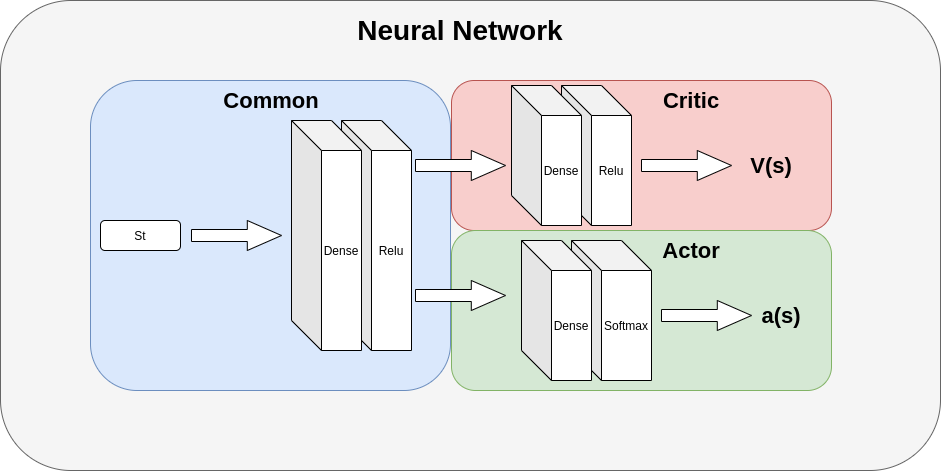
\includegraphics[width=0.5\textwidth]{imgs/network.png}
        \caption{\label{fig:method} Neural Network Structure}
    \end{figure}

As you can see the network is divided into two parts:
\begin{itemize}
    \item Critic 
    
    
    The Critic part is used to determine the value of the state in which the agent is in. 
    This part corresponds to the value-based part of the learning. It allows to stabilize the learning and to converge towards a global maximum of the policy.
    \item Actor
    
    
    The actor part corresponds to the part of the agent that takes action. It is the policy-based part of learning. 
    The actor part pulls out a probability distribution $\pi_{\theta}(s)$ which makes it possible to determine what probability is for the agent to take this or that action given the state.
  \end{itemize}
  The purpose of learning is to change the probability distribution in the direction that gives the maximum reward. 
  The value part allows to compare the quality of an action carried out in relation to the value of a state already estimated to know if this action is more optimised than what has been done before.


\subsection{Advantage Actor Critic algorithm}

To update the network parameters we used reinforcement learning. We used one of the most powerful reinforcement learning algorithms before the A3C. A2C is an algorithm halfway between value based learning and policy based learning.
\begin{figure}[!htb]
    \centering
    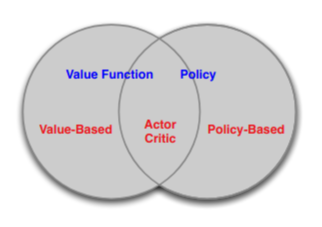
\includegraphics[width=0.3\textwidth]{imgs/actro.png}
    \caption{\label{fig:method} Actor Critic}
\end{figure}

The Advantage Actor Critic algorithm takes the following form :

\begin{figure}[!htb]
    \centering
    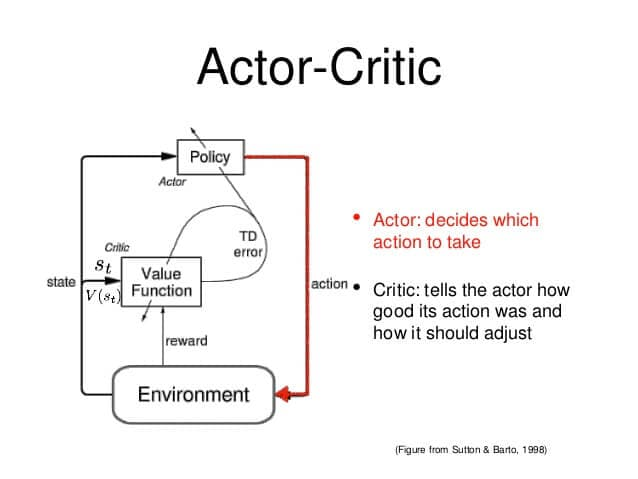
\includegraphics[width=0.5\textwidth]{imgs/actor_critic.jpeg}
    \caption{\label{fig:method} Actor Critic}
\end{figure}

\begin{algorithm}
\label{alga2c}
\caption{N-step Advantage Actor-Critic\label{a2c}}
\begin{algorithmic}[1]
\Procedure{N-Step Advantage Actor-Critic}{}
\State $\textit{Start with policy model } \pi_\theta \textit{ and value model } V_\omega$
\State $\textbf{repeat:}$
\State $\qquad\textit{Generate an episode } S_0, A_0, r_0, \ldots, S_{T-1}, A_{T-1}, r_{T-1} $
\State $\qquad\textbf{for } t \textit{ from } T-1 \textit{ to } 0$:
\State $\qquad\qquad V_{end} = 0 \text{ if } (t+N \geq T) \textit{ else } V_\omega(s_{t+N})$
\State $\qquad\qquad R_t =\gamma^{N}V_{end}+\sum_{k=0}^{N-1} \gamma^k \left(r_{t+k} \textit{ if } (t+k < T) \textit{ else } 0\right)$ 
\State $\qquad L(\theta) = \frac{1}{T} \sum_{i=0}^{T-1} (R_t - V_\omega(S_t)) \log \pi_\theta(A_t | S_t)$
\State $\qquad L(\omega) = \frac{1}{T} \sum_{i=0}^{T-1} (R_t - V_\omega(S_t))^2$
\State $\qquad\textit{Optimize } \pi_\theta \textit{ using } \nabla L(\theta)$
\State $\qquad\textit{Optimize } V_\omega \textit{ using } \nabla L(\omega)$
\EndProcedure
\end{algorithmic}
\end{algorithm}
As can be seen in figure 4, the principle of the critical actor is to take an action thanks to the actor and to criticise the action achieved thanks to the critic. But to criticise this action you need something to compare this action with the critic. This is the Advantage part. 
There are several ways of expressing Advantage.
But the most common method is to take as the advantage :  $Rt - V_{\pi_{\theta}(s,a)}$

with $Rt =\gamma^{N}V_{end}+\sum_{k=0}^{N-1} \gamma^k (r_{t+k})$.

As can be seen in figure 4, the advantage part of the algorithm can also be called the TD error.

In the literature one initially finds $Rt =\gamma V_{t+1}+r_{t}$
but recent work on replay experience has shown that taking into account more rewards makes it easier to converge towards a global minimum of the cost function estimating the MDP (Markovian decision process).
On the other hand, using this method implies a certain volatility of the estimator since a stock affects the value of a state further in time, and it often takes longer to converge.
It is therefore a question of finding the best hyper-parameters, which are often found empirically.

\subsection{Reward process}
In reinforcement learning methods the reward process is very important as it allows the robot to perceive its environment. 
More importantly, it corresponds to the MRP (Markovian reward process) that we try to estimate thanks to the neural network (the critical part). 
So if the reward process does not correspond exactly to the environment, the agent will not correctly estimate the behaviour it has to adopt.

